\documentclass[12pt, titlepage]{article}

\usepackage{graphicx} % Required for resizing the table

\usepackage{booktabs}
\usepackage{tabularx}
\usepackage{makecell}
\usepackage{hyperref}
\hypersetup{
    colorlinks,
    citecolor=black,
    filecolor=black,
    linkcolor=red,
    urlcolor=blue
}
\usepackage[round]{natbib}
\usepackage{longtable}
\usepackage{array}
\usepackage{float}

%% Comments

\usepackage{color}

\newif\ifcomments\commentstrue %displays comments
%\newif\ifcomments\commentsfalse %so that comments do not display

\ifcomments
\newcommand{\authornote}[3]{\textcolor{#1}{[#3 ---#2]}}
\newcommand{\todo}[1]{\textcolor{red}{[TODO: #1]}}
\else
\newcommand{\authornote}[3]{}
\newcommand{\todo}[1]{}
\fi

\newcommand{\wss}[1]{\authornote{blue}{SS}{#1}} 
\newcommand{\plt}[1]{\authornote{magenta}{TPLT}{#1}} %For explanation of the template
\newcommand{\an}[1]{\authornote{cyan}{Author}{#1}}

%% Common Parts

\newcommand{\progname}{ProgName} % PUT YOUR PROGRAM NAME HERE
\newcommand{\authname}{Team \#, Team Name
\\ Student 1 name
\\ Student 2 name
\\ Student 3 name
\\ Student 4 name} % AUTHOR NAMES                  

\usepackage{hyperref}
    \hypersetup{colorlinks=true, linkcolor=blue, citecolor=blue, filecolor=blue,
                urlcolor=blue, unicode=false}
    \urlstyle{same}
                                


\begin{document}

\title{Verification and Validation Report: \progname} 
\author{\authname}
\date{\today}
	
\maketitle

\pagenumbering{roman}

\section{Revision History}

\begin{tabularx}{\textwidth}{p{3cm}p{2cm}X}
  \toprule {\bf Date} & {\bf Version} & {\bf Notes}\\
  \midrule
  March 1 & 1.0 & Created Document Structure and Outline. Filled out most test cases and appendix reflection. \\
  March 8 & 1.1 & Unit Test report\\
  March 8 & 1.2 & Add more Unit Tests, System Tests, Reflection\\
  March 8 & 1.3 & Add test-requirement traceability\\
  \bottomrule
  \end{tabularx}

~\newpage

\section{Symbols, Abbreviations, and Acronyms}

\renewcommand{\arraystretch}{1.2}
\begin{tabular}{l l}
    \toprule
    \textbf{symbol} & \textbf{description}                                                  \\
    \midrule
    T               & Test                                                                  \\
    UT              & Unit Test                                                             \\
    RBAC            & Role-Based Access Control. Used for defining user permissions         \\
    UI              & User Interface                                                        \\
    JWT             & JSON Web Token. A compact way to transmit info securely               \\
    GSA             & Graduate Students' Association. The association overseeing the league \\
    SRS             & Software Requirements Specification                                   \\
    MIS             & Module Interface Specification                                        \\
    DD              & Design Document                                                       \\
    VnV             & Verification and Validation                                           \\
    CI              & Continuous Integration                                                \\
    API             & Application Programming Interface. Defines how software components interact \\
    CRUD            & Create, Read, Update, Delete. Basic operations for managing data      \\
    DB              & Database. A system for storing and managing data                      \\
    \bottomrule
\end{tabular}\\


\subsection{Symbolic Parameters}

The definition of the test cases will call for SYMBOLIC\_CONSTANTS.
Their values are defined in this section for easy maintenance.
\begin{longtable}{|l|l|l|p{5cm}|}
    \hline
    Parameter & Value & Unit & Description \\
    \hline
    \phantomsection\label{MAX_NAVTIME} \texttt{MAX\_NAVTIME} & 60 & s & The maximimum time acceptable for testers to navigate to a main view \\
    \hline
    \phantomsection\label{MIN_TESTERS} \texttt{MIN\_TESTERS} & 5 & n/a & The minimum number of testers required for a system test \\
    \hline
    \phantomsection\label{AVG_TASK_TIME} \texttt{AVG\_TASK\_TIME} & 3 & min & The average task time for a task completion \\
    \hline
    \phantomsection\label{MAX_GAME_DIFF} \texttt{MAX\_GAME\_DIFF} & 2 & n/a & The maximum difference in total scheduled games between two teams \\
    \hline
\end{longtable}

\newpage

\tableofcontents

\listoftables %if appropriate

\listoffigures %if appropriate

\newpage

\pagenumbering{arabic}

This document ...

\section{Functional Requirements Evaluation}

\subsection{Manual Testing}

\begin{enumerate}
    \item \textbf{FR-1}
          \begin{itemize}
              \item Description: Testing login functionality with wrong credentials.
              \item How Test Will Be Performed: Tester will attempt to log in with an invalid \texttt{UserID} and \texttt{Password}. Verify that all invalid logins are unsuccessful.
              \item Requirements Covered: SRS Req \#1 (authentication).
              \item Inputs: Invalid UserID and Password
              \item Expected Output: Failed to login
              \item Actual Output: Failed to login
              \item Result: Pass
          \end{itemize}

    \item \textbf{FR-2}
          \begin{itemize}
              \item Description: Testing login functionality with correct credentials.
              \item How Test Will Be Performed: Tester will log in with a valid \texttt{UserID} and \texttt{Password} for each \texttt{Role} (Player, Captain, Commissioner) and verify access to the platform after successful login under the correct account.
              \item Requirements Covered: SRS Req \#1 (authentication).
              \item Inputs: \texttt{UserID} and \texttt{Password} for valid commissioner, captain, and player accounts.
              \item Expected Output: Successful login for valid credentials.
              \item Actual Output: Successful login for valid credentials.
              \item Result: Pass
          \end{itemize}

       \item \textbf{FR-3}
          \begin{itemize}
              \item Description: Attempting to create a duplicate team name
              \item How Test Will be Performed: Tester will attempt to create a new team suing a duplicate \texttt{TeamName}. Verify that the team is not added to the database.
              \item Requirements Covered: SRS Req \#5 (team creation).
              \item Inputs: Enter a \texttt{TeamName} that already exists in the database and a Division.
              \item Expected Output: Unsuccessful creation of a team with a duplicate
              \item Actual Output: Unsuccessful creation of a team with a duplicate
              \item Result: Pass
          \end{itemize}

      \item \textbf{FR-4}  
      \begin{itemize}
          \item Description: Creating a new team with a unique name.
          \item How Test Will Be Performed: Tester will attempt to create a new team using a unique \texttt{TeamName} and Division. Verify that the team is successfully added to the database.
          \item Requirements Covered: SRS Req \#5 (team creation).
          \item Inputs: Enter a unique \texttt{TeamName} and Division.
          \item Expected Output: Successful team creation.
          \item Actual Output: Successful team creation.
          \item Result: Pass
      \end{itemize}

      \item \textbf{FR-5}  
      \begin{itemize}
          \item Description: Attempting to create multiple teams under one Captain.
          \item How Test Will Be Performed: Tester will attempt to create a second team while logged in as a Captain who already has an existing team. Verify that the new team is not added to the database.
          \item Requirements Covered: SRS Req \#5 (team creation).
          \item Inputs: Enter a new \texttt{TeamName} and Division while already associated with an existing team.
          \item Expected Output: Unsuccessful team creation. Error message displayed for multiple teams under one \texttt{CaptainID}.
          \item Actual Output: Not Tested Yet.
          \item Result: Not Tested Yet.
      \end{itemize}

      % \item \textbf{FR-6}  
      % \begin{itemize}
      %     \item Description: Player requesting to join a team.
      %     \item How Test Will Be Performed: Tester will attempt to join a team while logged in as a Player without an existing team. Verify that the associated Captain receives the request (Refer to FR-7).
      %     \item Requirements Covered: SRS Req \#6 (joining teams).
      %     \item Inputs: Player requests to join \texttt{TeamName}.
      %     \item Expected Output: Player’s request is sent to the team’s Captain.
      %     \item Actual Output: Player’s request is sent to the team’s Captain.
      %     \item Result: Pass
      % \end{itemize}

      % \item \textbf{FR-7}  
      % \begin{itemize}
      %     \item Description: Captain approving a player's join request.
      %     \item How Test Will Be Performed: Tester will log in as a Captain with an existing team and approve a pending player's join request. Verify that the team updates accordingly: Roster is updated in the database, and the player gains access to team-specific information.
      %     \item Requirements Covered: SRS Req \#6 (joining teams).
      %     \item Inputs: Captain receives and approves the request.
      %     \item Expected Output: \texttt{PlayerID} is added to the Roster of the team associated with \texttt{TeamName}.
      %     \item Actual Output: \texttt{PlayerID} is added to the Roster of the team associated with \texttt{TeamName}.
      %     \item Result: Pass
      % \end{itemize}

      \item \textbf{FR-7}  
      \begin{itemize}
          \item Description: Generating a season game schedule based on team availability and preferences.
          \item How Test Will Be Performed: Load the database with team availability, divisional assignments, game count requirements, and available slots. Run the schedule generation process. Refer to TPERF-2 for performance testing of the generated schedule.
          \item Requirements Covered: SRS Req \#7 (Schedule Automation).
          \item Inputs:  
              \begin{itemize}
                  \item Team Availability: Preferences for game days and times.  
                  \item Division Assignments: Each TeamID is assigned a division.  
                  \item Game Count Requirement: Ensures each team has an equal number of games.  
                  \item Available Slots: The availability of the event space.  
              \end{itemize}
          \item Expected Output: The system generates an appropriate season game schedule.
          \item Actual Output: The system successfully generates a season game schedule.
          \item Result: Pass
      \end{itemize}

    \item \textbf{FR-8}  
      \begin{itemize}
          \item Description: Captains submitting game results, which update the standings.
          \item How Test Will Be Performed: Captain submits game scores (ScoreTeamA, ScoreTeamB). Verify that the report is reflected in the database and that standings update accordingly.
          \item Requirements Covered: SRS Req \#12 (Reporting).
          \item Inputs:  
              \begin{itemize} 
                  \item ScoreTeamA: Score for Team A.  
                  \item ScoreTeamB: Score for Team B.  
              \end{itemize}
          \item Expected Output: Game report is updated, and standings reflect the new results.
          \item Actual Output: Game report successfully updates, and standings are correctly modified.
          \item Result: Pass
      \end{itemize}

      \item \textbf{FR-9}  
      \begin{itemize}
          \item Description: Captains submitting reschedule requests for approval by the Commissioner.
          \item How Test Will Be Performed: Captain initiates a reschedule request for an open slot. Verify that the request is sent to the Commissioner for approval.
          \item Requirements Covered: SRS Req \#8 (Rescheduling).
          \item Inputs:  
              \begin{itemize}
                  \item ScheduleID: Identifier for the current schedule.  
                  \item GameID: Identifier for the game being rescheduled.  
                  \item SlotNumber: Open slot requested for rescheduling.  
              \end{itemize}
          \item Expected Output: Request is successfully sent to the Commissioner for review.
          \item Actual Output: Not Tested Yet.
          \item Result: Not Tested Yet.
      \end{itemize}

    \item \textbf{FR-10}  
      \begin{itemize}
          \item Description: Commissioner overriding a scheduled game (cancel or reschedule) or approving a reschedule request.
          \item How Test Will Be Performed: Commissioner applies an override on an existing game. Verify that the schedule updates correctly (Schedule view, SlotNumber, and Available Slots). Confirm that notifications are sent to all affected team members.
          \item Requirements Covered: SRS Req \#11 (Game Overrides).
          \item Inputs:  
              \begin{itemize}
                  \item GameID: Identifier for the game being overridden.  
                  \item Override Type: Cancel or reschedule.  
                  \item New SlotNumber (if rescheduling): The newly assigned game slot.  
              \end{itemize}
          \item Expected Output: The override is reflected in the schedule, and all rostered team members receive notifications.
          \item Actual Output: Not Tested Yet.
          \item Result: Not Tested Yet.
      \end{itemize}

      \item \textbf{FR-11}  
      \begin{itemize}
          \item Description: Commissioner posts a league-wide announcement that should be visible across all platform views.
          \item How Test Will Be Performed: Commissioner submits an announcement. Verify that the announcement is displayed to all users across the platform.
          \item Requirements Covered: SRS Req \#9, \#10 (Announcements).
          \item Inputs:  
              \begin{itemize}
                  \item Announcement Title: The subject of the announcement.
                  \item Announcement Body: The message content.
                  \item Visibility Scope: League-wide.
              \end{itemize}
          \item Expected Output: Announcement is displayed across all platform views and is accessible to all users.
          \item Actual Output: Announcement successfully visible to all users.
          \item Result: Pass
      \end{itemize}
\end{enumerate}

\subsection{System Testing}
\begin{enumerate}
    \item \textbf{FR-1}
    \begin{itemize}
        \item \textbf{Description:} Test login functionality with valid credentials.
        \item \textbf{Test Method:} Automated test using \texttt{playerControllers.test.js} to create a player account and log in with valid credentials for each \texttt{Role} (Player, Captain, Commissioner).
        \item \textbf{Expected Result:} Successful login for each role and access to platform functionalities.
        \item \textbf{Result:} Pass
    \end{itemize}

    \item \textbf{FR-2}
        \begin{itemize}
            \item Description: Testing login functionality with correct credentials.
            \item How Test Will Be Performed: A backend script in `playerControllers.test.js' will create a Player account with a \texttt{UserID} and \texttt{Password}. The tester will log in with a valid \texttt{UserID} and \texttt{Password} for each \texttt{Role} (Player, Captain, Commissioner) and verify access to the platform after successful login under the correct account. Test data will be created in the database and cleaned up after the test.
            \item Requirements Covered: SRS Req \#1 (authentication).
            \item Result: Pass
        \end{itemize}

        \item \textbf{FR-3}
        \begin{itemize}
            \item \textbf{Description:} Create a new team with a unique name.
            \item \textbf{Test Method:} Automated test using \texttt{teamControllers.test.js} to input a unique \texttt{TeamName} and Division, and create a team.
            \item \textbf{Expected Result:} The team should be successfully added to the database.
            \item \textbf{Result:} Pass
        \end{itemize}

    \item \textbf{FR-4}  
    \begin{itemize}
        \item \textbf{Description:} Create a new team with an existing name.
        \item \textbf{Test Method:} Automated test using \texttt{teamControllers.test.js} to input an exisiting \texttt{TeamName} and Division, and create a team.
        \item \textbf{Expected Result:} The team should be successfully added to the database.
        \item \textbf{Result:} Fail
    \end{itemize}
    \item \textbf{FR-5}  
    \begin{itemize}
        \item \textbf{Description:} Test system behavior when attempting to create multiple teams under a single Captain.
        \item \textbf{Test Method:} Automated test using \texttt{teamControllers.test.js} to create multiple teams under one Captain and verify error handling.
        \item \textbf{Expected Result:} The second team should not be created, and an error message should appear.
        \item \textbf{Result:} Fail 
    \end{itemize}
\end{enumerate}

\section{Nonfunctional Requirements Evaluation}

\subsection{Usability}

\subsubsection{Usability Survey Results}

As part of our usability evaluation, we conducted a survey with participants who tested the platform for the first time. Testers were asked to complete key tasks such as signing up, logging in, creating a team, requesting reschedules, and navigating the interface. After completing these tasks, they provided feedback via a post-task survey.\\

The full survey can be accessed at:  
\href{https://docs.google.com/forms/d/e/1FAIpQLSeJ6XQhV2XkQ3CwSQN0GmwiXQIoUg9fHRQ2i7hpc-1skot2jQ/viewform}{Google Forms Usability Survey}.\\


Table \ref{tab:usabilitySurvey} summarizes the responses of \hyperref[MIN_TESTERS]{\texttt{MIN\_TESTERS}} participants (Response IDs 0--4) to our usability questionnaire. Each row corresponds to one survey question.

\begin{longtable}{|p{0.25\textwidth}|
    >{\raggedright\arraybackslash}p{0.11\textwidth}|
    >{\raggedright\arraybackslash}p{0.14\textwidth}|
    >{\raggedright\arraybackslash}p{0.11\textwidth}|
    >{\raggedright\arraybackslash}p{0.11\textwidth}|
    >{\raggedright\arraybackslash}p{0.11\textwidth}|}
\caption{Usability Survey Questions and Responses (Updated Data)}
\label{tab:usabilitySurvey}\\

\hline
\textbf{Question} & \textbf{Resp.\ 0} & \textbf{Resp.\ 1} & \textbf{Resp.\ 2} & \textbf{Resp.\ 3} & \textbf{Resp.\ 4}\\
\hline
\endfirsthead

\multicolumn{6}{r}{\bfseries Table \thetable\ (continued)}\\
\hline
\textbf{Question} & \textbf{Resp.\ 0} & \textbf{Resp.\ 1} & \textbf{Resp.\ 2} & \textbf{Resp.\ 3} & \textbf{Resp.\ 4}\\
\hline
\endhead

\hline
\multicolumn{6}{r}{\textit{Continued on next page}}\\
\hline
\endfoot

\hline
\endlastfoot

%------------------------------------------------------------------------------------
% Q1
How easy was it to learn how to use the platform?
& 5
& 4
& 5
& 5
& 5 \\ \hline

% Q2
How confident do you feel using the platform without assistance after your initial experience?
& 5
& 5
& 5
& 5
& 5 \\ \hline

% Q3
How intuitive do you find the navigation of the platform?
& 5
& 5
& 5
& 5
& 5 \\ \hline

% Q4
How long did it take you to navigate all the views? (Approx.\ in minutes)
& 3
& 5
& 2
& 2
& 3 \\ \hline

% Q5
How easy was it to complete basic tasks (login, create team, request reschedule)?
& 4
& 4
& 5
& 5
& 5 \\ \hline

% Q6
Did you encounter any errors or issues while using the platform? If so, please describe them.
& \parbox[t]{0.11\textwidth}{\raggedright \textit{(none)}}
& \parbox[t]{0.11\textwidth}{\raggedright Invalid email accepted.  Misspelled @gmail.com and it still allowed it.}
& \parbox[t]{0.11\textwidth}{\raggedright \textit{(none)}}
& \parbox[t]{0.11\textwidth}{\raggedright NA}
& \parbox[t]{0.11\textwidth}{\raggedright \textit{(none)}} \\ \hline

% Q7
How helpful were the in-app help resources in learning how to use the platform?
& 5
& 5
& 3
& 5
& 5 \\ \hline

% Q8
Please share any suggestions for improving the in-app help resources.
& 4
& \parbox[t]{0.11\textwidth}{\raggedright \textit{(none)}}
& \parbox[t]{0.11\textwidth}{\raggedright i didn't need them}
& \parbox[t]{0.11\textwidth}{\raggedright NA}
& \textit{(none)} \\ \hline

% Q9
Did the platform's interface appear modern, intuitive, and visually consistent across all views?
& \parbox[t]{0.11\textwidth}{\raggedright the use of yellow randomly appears only in a couple pages}
& 4
& 5
& 5
& 5 \\ \hline

% Q10
Did you observe any remarkable inconsistencies in the visual interface when navigating (login, team mgmt, schedule)?
& \parbox[t]{0.11\textwidth}{\raggedright the use of yellow randomly appears only in a couple pages}
& \parbox[t]{0.11\textwidth}{\raggedright \textit{(none)}}
& \parbox[t]{0.11\textwidth}{\raggedright \textit{(none)}}
& \parbox[t]{0.11\textwidth}{\raggedright NA}
& \parbox[t]{0.11\textwidth}{\raggedright maybe some fonts} \\ \hline

% Q11
How accessible do you find the platform in terms of visual design (color contrast, text size, font)?
& 4
& 5
& 5
& 5
& 5 \\ \hline

% Q12
Do you have any suggestions for improving the accessibility of the platform?
& \parbox[t]{0.11\textwidth}{\raggedright yellow might be hard for some people to see}
& \parbox[t]{0.11\textwidth}{\raggedright \textit{(none)}}
& \parbox[t]{0.11\textwidth}{\raggedright maybe bigger fonts in some places}
& \parbox[t]{0.11\textwidth}{\raggedright NA}
& \parbox[t]{0.11\textwidth}{\raggedright \textit{(none)}} \\ \hline

% Q13
Based on the Canadian formatting standards provided, do you believe the platform adheres to these conventions?
& Yes
& Yes
& Yes
& Yes
& Yes \\ \hline

% Q14
If you noticed any deviations from Canadian formatting standards, please describe them.
& \parbox[t]{0.11\textwidth}{\raggedright \textit{(none)}}
& \parbox[t]{0.11\textwidth}{\raggedright \textit{(none)}}
& \parbox[t]{0.11\textwidth}{\raggedright \textit{(none)}}
& \parbox[t]{0.11\textwidth}{\raggedright NA}
& \parbox[t]{0.11\textwidth}{\raggedright i didn't notice} \\ \hline

% Q15
Would you like to provide any additional comments on your experience?
& \parbox[t]{0.11\textwidth}{\raggedright \textit{(none)}}
& \parbox[t]{0.11\textwidth}{\raggedright I like overall that the colours adhere to McMaster}
& \parbox[t]{0.11\textwidth}{\raggedright super easy to use}
& \parbox[t]{0.11\textwidth}{\raggedright NA}
& \parbox[t]{0.11\textwidth}{\raggedright i like it a lot} \\ \hline

\end{longtable}

The usability survey results indicate that the platform is highly intuitive and easy for new users to learn and navigate. The responses were overwhelmingly positive, with all participants successfully completing tasks such as signing up, logging in, and exploring key sections of the site. Navigation times were within the expected range, and testers generally found the interface modern, visually consistent, and user-friendly.

One minor concern was that a participant rated the in-app help resources lower than others. However, this response likely reflects the fact that the help resources were unnecessary rather than inadequate, which is ultimately a positive outcome. Another issue noted was an invalid email being accepted during sign-up. While this can be corrected in the edit profile feature, the team will consider implementing stricter validation on the registration page to prevent similar cases.

Overall, the results confirm that the platform meets usability expectations and is on track for successful deployment, with only minor refinements needed for edge cases.



\subsubsection{Manual Testing}
\begin{enumerate}
\item \textbf{TUH-1}  
      \begin{itemize}
          \item Description: Evaluate ease of navigation for new users by measuring time taken to access key platform views.
          \item How Test Will Be Performed: Conduct an observational usability study where participants navigate through login, announcements, standings, and schedule pages. Record navigation times and collect feedback through a post-task survey.
          \item Requirements Covered: SRS Req \#11.1 (Usability - Navigation).
          \item Inputs:  
              \begin{itemize}
                  \item Navigation Tasks: Tester navigates through login, announcements, standings, and schedule pages.
                  \item Participants: \hyperref[MIN_TESTERS]{\texttt{MIN\_TESTERS}} with no prior experience with the platform.
              \end{itemize}
          \item Expected Output: Participants successfully navigate to each view within \hyperref[MAX_NAVTIME]{\texttt{MAX\_NAVTIME}} without prior experience or external assistance.
          \item Actual Output: Participants completed navigation within the expected time.
          \begin{figure}[h!]
            \centering
            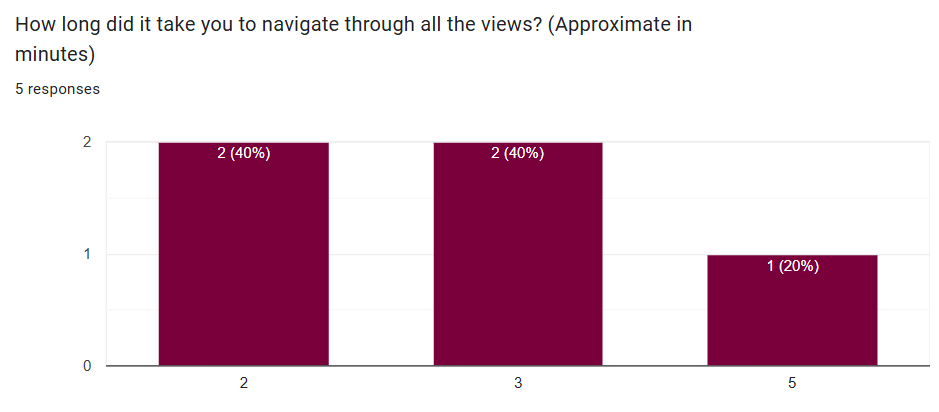
\includegraphics[width=1\textwidth]{navtime_results.png}
            \caption{Survey results showing participants' average navigation times.}
            \label{fig:navtime}
          \end{figure}
          \item Result: Pass
      \end{itemize}

    \item \textbf{TUH-2}  
    \begin{itemize}
        \item Description: Verify the platform displays date, time, and measurements according to Canadian localization standards.
        \item How Test Will Be Performed: Verify date, time, and measurement units across the platform views. Ask usability testers to confirm that information formats are clear and match Canadian standards. Feedback survey included in Appendix.
        \item Requirements Covered: SRS Req \#11.2 (Localization - Canadian Standards).
        \item Inputs:  
            \begin{itemize}
                \item Date, Time, and Measurement Fields: Tester reviews the date, time, and metric system information across the platform.
                \item Participants: Usability testers verify format clarity and standard compliance.
            \end{itemize}
        \item Expected Output: Platform displays date and time in Canadian format, uses the metric system, and all text is in Canadian English.
        \item Actual Output: Not Tested Yet.
        \item Result: Not Tested Yet.
    \end{itemize}

    \item \textbf{TUH-3}  
    \begin{itemize}
        \item Description: Evaluate the effectiveness of in-app learning support by measuring how quickly new users can complete tasks using the platform’s guidance tools.
        \item How Test Will Be Performed: Conduct an observational usability study with \hyperref[MIN_TESTERS]{\texttt{MIN\_TESTERS}} participants who have no prior experience with the platform. Record the time taken for each task completion. Following the tasks, participants will complete a survey (in Appendix) to provide feedback on task difficulty and provided guidance.
        \item Requirements Covered: SRS Req \#11.3-11.4 (Usability - Task Completion and Learning Support).
        \item Inputs:  
            \begin{itemize}
                \item Tasks: Tester performs login, creates a team, and requests a reschedule.
                \item Participants: \hyperref[MIN_TESTERS]{\texttt{MIN\_TESTERS}} with no prior experience with the platform.
            \end{itemize}
        \item Expected Output: Tester completes each task within an average of \hyperref[AVG_TASK_TIME]{\texttt{AVG\_TASK\_TIME}} minutes, utilizing in-app guidance (navigation instructions, tooltips, help documentation) to easily understand and complete tasks.
        \item Actual Output: Tester completed each task within the expected time and used in-app help effectively.
        \begin{figure}[H]
            \centering
            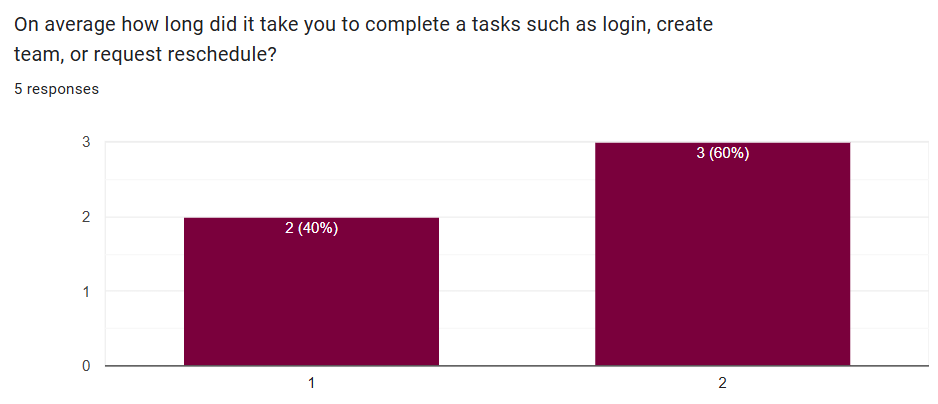
\includegraphics[width=1\textwidth]{avg_task_results.png}
            \caption{Survey results showing participants' average task completion times.}
            \label{fig:navtime}
        \end{figure}
        \item Result: Pass
    \end{itemize}
\end{enumerate}
		
\subsection{Performance}

\subsubsection{Manual Testing}
\begin{enumerate}
    \item \textbf{TPERF-1}  
        \begin{itemize}
            \item Description: Verify the accuracy of the league standings calculations.
            \item How Test Will Be Performed: Create test cases with predefined standings. Use an automated script to perform calculations and check results against expected outcomes, ensuring all calculations are accurate.
            \item Requirements Covered: SRS Req \#12.1, 12.3 (Performance - Standings Calculation Accuracy).
            \item Inputs:  
                \begin{itemize}
                    \item Sample Data: Predefined standings data for the league.
                    \item Tester: Automated script performing the calculation checks.
                \end{itemize}
            \item Expected Output: The standings are calculated with 100% accuracy, as outlined in the functional requirements.
            \item Actual Output: The standings were calculated with 100% accuracy.
            \item Result: Pass
        \end{itemize}

\item \textbf{TPERF-2}  
    \begin{itemize}
        \item Description: Verify the accuracy and balance of the league schedule, ensuring that teams play within their division, with balanced game counts, and no conflicts.
        \item How Test Will Be Performed: The platform is prepared with a sample dataset containing multiple teams and generates a schedule. The tester manually verifies the schedule, checking that each team is assigned games within the schedule, ensuring a balanced number of games, verifying divisional match-ups, and logging any conflicts.
        \item Requirements Covered: SRS Req \#12.4 (Performance - Scheduling Accuracy and Optimization).
        \item Inputs:  
            \begin{itemize}
                \item Sample Data: Teams and their preferences for scheduling.
                \item Tester: Manually verifying the schedule.
            \end{itemize}
        \item Expected Output:  
            \begin{itemize}
                \item The displayed schedule shows that all teams have a balanced number of scheduled games, with no team having a game count differing by more than \hyperref[MAX_GAME_DIFF]{\texttt{MAX\_GAME\_DIFF}} games from any other team.
                \item The displayed schedule shows that all teams play 100% of their games within their division.
                \item The displayed schedule is conflict-free, considering time and location.
                \item The displayed schedule is optimized based on matching team preferences.
            \end{itemize}
        \item Actual Output: Not Tested Yet.
        \item Result: Not Tested Yet.
    \end{itemize}

 \item \textbf{TPERF-3}  
    \begin{itemize}
        \item Description: Verify that new login credentials are properly added and stored in the database.
        \item How Test Will Be Performed: The tester manually adds a pair of new credentials and checks whether the information is stored correctly in the database.
        \item Requirements Covered: SRS Req \#12.2 (Performance - Credential Storage).
        \item Inputs:  
            \begin{itemize}
                \item New Login Credentials: A pair of new user credentials to be added to the system.
                \item Tester: Manually verifying the database storage.
            \end{itemize}
        \item Expected Output: The credentials are stored in the database in the correct format.
        \item Actual Output: The credentials were stored in the database in the correct format.
        \item Result: Pass
    \end{itemize}

\item \textbf{TPERF-4}  
    \begin{itemize}
        \item Description: Verify that the platform handles invalid form submissions by highlighting errors and preventing submission until corrections are made.
        \item How Test Will Be Performed: Testers will intentionally leave required fields blank, enter invalid data formats, and submit the form. Testers will verify that the fields with errors are highlighted visually and that informative error messages appear next to the problematic fields, indicating the nature of the errors. Testers will confirm that the information in the form is not submitted into the database until the errors are corrected and the form is resubmitted, showing a success message upon submission.
        \item Requirements Covered: SRS Req \#12.4 (Performance - Form Validation and Error Handling).
        \item Inputs:  
            \begin{itemize}
                \item Invalid Data: Required fields left blank, incorrect data formats (e.g., invalid email).
                \item Tester: Manually interacting with the form and submitting.
            \end{itemize}
        \item Expected Output:  
            \begin{itemize}
                \item Fields with errors are highlighted visually.
                \item Informative error messages appear next to the problematic fields.
                \item Form submission is prevented until all errors are corrected.
                \item A success message appears upon a successful resubmission after error correction.
            \end{itemize}
        \item Actual Output: Not Tested Yet.
        \item Result: Not Tested Yet.
    \end{itemize}

\end{enumerate}

\subsection{Operational and Environmental}
\subsubsection{Manual Testing}
\begin{enumerate}
    \item \textbf{TOPE-1}  
    \begin{itemize}
        \item Description: Verify that the platform is fully accessible and functional across desktop, tablet, and smartphone devices.
        \item How Test Will Be Performed: Perform manual testing of the platform features, responsiveness, and navigation on desktop, tablet, and smartphone. Ensure all features are accessible and function correctly on each device type.
        \item Requirements Covered: SRS Req \#13.1 (Platform Compatibility - Multi-Device Accessibility).
        \item Inputs:  
            \begin{itemize}
                \item Device Types: Desktop, tablet, and smartphone.
                \item Tester: Manually interacting with the platform across all device types.
            \end{itemize}
        \item Expected Output: The platform is fully accessible and functional on all device types, with no loss of features or navigation issues.
        \item Actual Output: Not Tested Yet.
        \item Result: Not Tested Yet.
    \end{itemize}

    \item \textbf{TOPE-2}  
    \begin{itemize}
        \item Description: Verify that the platform is compatible and displays correctly across major browsers (Chrome, Firefox, Safari, and Edge).
        \item How Test Will Be Performed: Testers manually access all features and views of the platform in each of the browsers (Chrome, Firefox, Safari, and Edge). Ensure that the platform displays correctly and functions as expected in each browser.
        \item Requirements Covered: SRS Req \#13.2-13.3 (Browser Compatibility).
        \item Inputs:  
            \begin{itemize}
                \item Browser Types: Chrome, Firefox, Safari, and Edge.
                \item Tester: Manually interacting with the platform across each browser.
            \end{itemize}
        \item Expected Output: The platform displays correctly across all major browsers, with no visual or functional issues.
        \item Actual Output: Not Tested Yet.
        \item Result: Not Tested Yet.
    \end{itemize}
\end{enumerate}

\subsection{Maintainability and Support}
\subsubsection{Manual Testing}
\begin{enumerate}
    \item \textbf{TMS-1}  
    \begin{itemize}
        \item Description: Verify that users can contact support via email without any external assistance.
        \item How Test Will Be Performed: A minimum number of testers (\hyperref[MIN_TESTERS]{\texttt{MIN\_TESTERS}}) will be asked to reach support through email. Testers will document any difficulties encountered during the process.
        \item Requirements Covered: SRS Req \#14.1, 14.2 (Support - Contact Mechanism).
        \item Inputs:  
            \begin{itemize}
                \item Support Email: The email address to contact support.
                \item Tester: Manually sending an email to the support team.
            \end{itemize}
        \item Expected Output: The support team receives the help request from the tester via email, with no external help required.
        \item Actual Output: Not Tested Yet.
        \item Result: Not Tested Yet.
    \end{itemize}
\end{enumerate}

\subsection{Security}
\subsubsection{Manual Testing}
\begin{enumerate}
    \item \textbf{TSEC-1}  
    \begin{itemize}
        \item Description: Verify that users with different roles (Player, Captain, Commissioner) have the appropriate level of access to platform features.
        \item How Test Will Be Performed: Manually log in with a dummy user for each role (Administrator, Team Manager, Player, and Captain). Attempt to access various features and verify that the access levels match the defined role-based access control requirements.
        \item Requirements Covered: SRS Req \#15.1, 15.2 (Security - Role-Based Access Control).
        \item Inputs:  
            \begin{itemize}
                \item User Roles: Administrator, Team Manager, Player, and Captain.
                \item Tester: Manually logging in with each role and testing access to platform features.
            \end{itemize}
        \item Expected Output:  
            \begin{itemize}
                \item The Player role has restricted access, with only basic features (e.g., viewing schedule, joining teams).
                \item The Captain role has access to additional team management features.
                \item The Commissioner has access to all administrative features.
            \end{itemize}
        \item Actual Output: Not Tested Yet.
        \item Result: Not Tested Yet.
    \end{itemize}

    % \item \textbf{TSEC-2}  
    % \begin{itemize}
    %     \item Description: Verify that the platform prevents submission of invalid data and displays appropriate error messages.
    %     \item How Test Will Be Performed: Enter invalid data into the respective forms (e.g., team roster with missing player names, invalid team or game information) and submit. Observe the system's responses to ensure that appropriate validation messages are displayed and that no invalid data is submitted or saved to the database.
    %     \item Requirements Covered: SRS Req \#15.1, 15.2 (Security - Data Validation and Error Handling).
    %     \item Inputs:  
    %         \begin{itemize}
    %             \item Invalid Data: Examples include missing player names, incorrect team or game information.
    %             \item Tester: Manually entering invalid data into the forms and submitting.
    %         \end{itemize}
    %     \item Expected Output: The system should display helpful error messages and prevent the submission of invalid data, ensuring that no incorrect data is saved to the database.
    %     \item Actual Output: The system correctly prevented data submission for invalid inputs and displayed error messages.
    %     \item Result: Pass
    % \end{itemize}
\end{enumerate}

\subsection{Cultural}
\subsubsection{Manual Testing}
\begin{enumerate}
    \item \textbf{TCU-1}  
    \begin{itemize}
        \item Description: Verify that all text is displayed in Canadian English and the time is shown in the correct Hamilton, Ontario, Canada time zone (EST).
        \item How Test Will Be Performed: Manually inspect the platform's content, ensuring that all text is displayed in Canadian English and that date/time formats reflect the Hamilton, Ontario time zone (EST).
        \item Requirements Covered: SRS Req \#16.1 (Content - Localization and Time Zone).
        \item Inputs:  
            \begin{itemize}
                \item Platform Content: Text, date, and time information.
                \item Tester: Manually inspecting the platform for correctness in language and time zone.
            \end{itemize}
        \item Expected Output: All text is displayed in Canadian English, and time is correctly displayed in EST (Hamilton, Ontario).
        \item Actual Output: The platform displayed all content in Canadian English, with the correct time zone.
        \item Result: Pass
    \end{itemize}

\end{enumerate}

\subsection{Compliance}
\subsubsection{Manual Testing}
\begin{enumerate}
    \item \textbf{TC-1}  
    \begin{itemize}
        \item Description: Verify that a user can delete their account and associated personal data, and receive confirmation of deletion.
        \item How Test Will Be Performed: Manually delete a dummy user account and verify that all associated personal data (e.g., email, phone number) is removed from the database and platform. Log any unexpected time elapsed to ensure the deletion process is secure and compliant with expected time frames.
        \item Requirements Covered: SRS Req \#17.1 (Functional - Data Deletion and Compliance).
        \item Inputs:  
            \begin{itemize}
                \item User Account: Dummy account with personal data (email, phone number).
                \item Tester: Initiating the account deletion request.
            \end{itemize}
        \item Expected Output: All personal data associated with the account is removed from the database and platform, and the user receives confirmation of successful deletion.
        \item Actual Output: Not Tested Yet.
        \item Result: Not Tested Yet.
    \end{itemize}

    \item \textbf{TC-2}  
    \begin{itemize}
        \item Description: Verify that the platform adheres to W3C web standards, including readable fonts, accessible colors, and clear navigation.
        \item How Test Will Be Performed: Manually inspect the platform's interface to ensure compliance with W3C web standards, focusing on font readability, color contrast, and navigation clarity.
        \item Requirements Covered: SRS Req \#17.2 (Functional - Web Standards Compliance).
        \item Inputs:  
            \begin{itemize}
                \item Platform Interface: The visual elements of the platform, including text, colors, and navigation.
                \item Tester: Manually inspecting the platform against W3C standards.
            \end{itemize}
        \item Expected Output: The platform meets W3C standards for font readability, accessible color contrasts, and clear navigation.
        \item Actual Output: The platform adheres to the W3C web standards.
        \item Result: Pass
    \end{itemize}

\end{enumerate}
	
\section{Comparison to Existing Implementation}	

Existing Implementation: \href{https://www.gsasoftball.ca/}{GSA Softball Website}

    \begin{itemize}
        \item \textbf{User Experience:} Our platform provides a more intuitive and streamlined navigation experience, with easy-to-find features like schedules, team management, and announcements.
        \item \textbf{Design and Aesthetics:} Our site boasts a modern, responsive design that adapts seamlessly across devices, offering a clean and visually appealing interface.
        \item \textbf{Functionality:} We provide advanced features such as live score updates, team rosters, and user-specific dashboards, which are absent or less efficient on the existing site.
        % \item \textbf{Performance:} Our site is optimized for faster load times and smoother interactions, enhancing the overall user experience.
        \item \textbf{Accessibility:} We prioritize accessibility, ensuring that the site is usable for individuals with disabilities, with features like screen reader compatibility and improved color contrast.
         \item \textbf{Team Page View:} Unlike the old website, our website allows users to view their team information on a "my team" page, which allows for easy access to useful information.
         \item \textbf{Game Scores:} Unlike the old website, the user had to manually fill out a game form and send it to the commissioner. Our new implementation allows captains to fill out the scores quickly and submit in less than a couple seconds.
    \end{itemize}

\section{Unit Testing}

\subsection{Current Backend Unit Testing}

Our current backend unit testing aligns closely with our VnV Plan for unit testing. We opted to start by unit testing the backend models in order to ensure that the foundational components of our platform are reliable and follow our requirements so that we can build more complex features with confidence.

Some tests were added since the VnVPlan was created and some tests were removed and are to be tested in integration testing.

Our backend unit testing is conducted using Jest and executed via npm test in the backend directory. The test files are located in the backend/test folder. These unit tests focus on verifying the fundamental functionality of our backend models, ensuring they behave as expected when interacting with MongoDB.

We began with backend testing because any issues caused by front-end components would be reflected in the backend models. By starting with the backend, we can ensure that the core functionality of our platform is reliable and that we can build more complex features with confidence.

Tests for Season, Reschedule Request, Announcements are WIP and some of their tests are documented below, but were not part of the VnVPlan.

\subsubsection{Player Model}

\begin{enumerate}
    \item{\textbf{test-player-creation}\\}
        \textbf{Path:} backend/test/models/playerTests.test.js\\
        \textbf{Description:} Verify that the player model can be created with valid input and default fields are set correctly.\\
        \textbf{Result:} Pass

    \item{\textbf{test-player-uniqueness}\\}
        \textbf{Path:} backend/test/models/playerTests.test.js\\
        \textbf{Description:} Verify that the player model enforces uniqueness for the email field.\\
        \textbf{Result:} Pass
\end{enumerate}
\subsubsection{Team Model}
\begin{enumerate}
    \item{\textbf{test-team-creation}\\}
        \textbf{Path:} backend/test/models/teamTests.test.js\\
        \textbf{Description:} Verify that the team model can be created with valid input, and default fields are set correctly.\\
        \textbf{Result:} Pass

    \item{\textbf{test-team-invalid-fields}\\}
        \textbf{Path:} backend/test/models/teamTests.test.js\\
        \textbf{Description:} Verify that attempting to create a team with missing or invalid fields fails validation.\\
        \textbf{Result:} Pass
\end{enumerate}

\textbf{Note:} Team uniqueness (VnVPlan test-team-uniqueness) will be verified as part of integration testing rather than unit testing.
\subsubsection{Game Model}
\begin{enumerate}
    \item{\textbf{test-game-creation}\\}
        \textbf{Path:} backend/test/models/gameTests.test.js\\
        \textbf{Description:} Verify that a Game can be created with valid input and default fields are set correctly (scores defaults to 0).\\
        \textbf{Result:} Pass
\end{enumerate}

\subsubsection{Gameslot Model}
\begin{enumerate}
    \item{\textbf{test-gameslot-creation}\\}
        \textbf{Path:} backend/test/models/gameslotTests.test.js\\
        \textbf{Description:} Verify that a game slot can be created with valid input, ensuring all required fields are properly stored.\\
        \textbf{Result:} Pass

    \item{\textbf{test-gameslot-uniqueness}\\}
        \textbf{Path:} backend/test/models/gameslotTests.test.js\\
        \textbf{Description:} Verify that a game slot enforces uniqueness based on date, time, and field to prevent duplicate entries.\\
        \textbf{Result:} Pass
\end{enumerate}

\subsubsection{Schedule Model}
\begin{enumerate}
    \item{\textbf{test-schedule-creation}\\}
        \textbf{Path:} backend/test/models/scheduleTests.test.js\\
        \textbf{Description:} Verify that a schedule can be created with the required fields, including \texttt{seasonId}, \texttt{gameSlots}, and \texttt{games}.\\
        \textbf{Result:} Pass

    \item{\textbf{test-schedule-timestamps}\\}
        \textbf{Path:} backend/test/models/scheduleTests.test.js\\
        \textbf{Description:} Verify that a schedule model includes automatically generated timestamps (\texttt{createdAt} and \texttt{updatedAt}).\\
        \textbf{Result:} Pass
\end{enumerate}

\subsubsection{Reschedule Request Model}
    \begin{enumerate}\item{\textbf{test-reschedule-request-missing-required-fields}\\}
        \textbf{Path:} backend/test/models/rescheduleRequestTests.test.js\\
        \textbf{Description:} Verify that missing required fields such as \texttt{game}, \texttt{requestingTeam}, \texttt{recipientTeam}, or \texttt{requestedGameslot} result in validation errors.\\
        \textbf{Result:} Pass

    \item{\textbf{test-reschedule-request-default-status}\\}
        \textbf{Path:} backend/test/models/rescheduleRequestTests.test.js\\
        \textbf{Description:} Verify that the \texttt{status} field defaults to \texttt{Pending} when no status is provided.\\
        \textbf{Result:} Pass

    \item{\textbf{test-reschedule-request-valid-status}\\}
        \textbf{Path:} backend/test/models/rescheduleRequestTests.test.js\\
        \textbf{Description:} Verify that the \texttt{status} field accepts valid values, including \texttt{Accepted}, \texttt{Pending}, and \texttt{Declined}.\\
        \textbf{Result:} Pass

    \item{\textbf{test-reschedule-request-invalid-status}\\}
        \textbf{Path:} backend/test/models/rescheduleRequestTests.test.js\\
        \textbf{Description:} Verify that invalid values for the \texttt{status} field, such as \texttt{InvalidStatus}, throw a validation error.\\
        \textbf{Result:} Pass

    \item{\textbf{test-reschedule-request-timestamps}\\}
        \textbf{Path:} backend/test/models/rescheduleRequestTests.test.js\\
        \textbf{Description:} Verify that the \texttt{createdAt} and \texttt{updatedAt} fields are automatically set by the Mongoose schema when a reschedule request is created.\\
        \textbf{Result:} Pass
\end{enumerate}

\subsubsection{Announcement Model}
\begin{enumerate}
        \item{\textbf{test-announcement-missing-required-fields}\\}
        \textbf{Path:} backend/test/models/announcementTests.test.js\\
        \textbf{Description:} Verify that missing required fields such as \texttt{title} or \texttt{content} result in validation errors.\\
        \textbf{Result:} Pass

    \item{\textbf{test-announcement-content-validation}\\}
        \textbf{Path:} backend/test/models/announcementTests.test.js\\
        \textbf{Description:} Verify that the \texttt{content} field is required and cannot be empty.\\
        \textbf{Result:} Pass

    \item{\textbf{test-announcement-timestamps}\\}
        \textbf{Path:} backend/test/models/announcementTests.test.js\\
        \textbf{Description:} Verify that the \texttt{createdAt} field is automatically set when an announcement is created.\\
        \textbf{Result:} Pass
\end{enumerate}

\subsubsection{Season Model}
\begin{enumerate}
    \item{\textbf{test-season-unique-name}\\}
    \textbf{Path:} backend/test/models/seasonTests.test.js\\
    \textbf{Description:} Verify that the \texttt{name} field is unique, ensuring no two seasons can have the same name.\\
    \textbf{Result:} Pass

    \item{\textbf{test-season-default-allowedDivisions}\\}
        \textbf{Path:} backend/test/models/seasonTests.test.js\\
        \textbf{Description:} Verify that the \texttt{allowedDivisions} field defaults to \texttt{4} when not provided.\\
        \textbf{Result:} Pass

    \item{\textbf{test-season-missing-required-fields}\\}
        \textbf{Path:} backend/test/models/seasonTests.test.js\\
        \textbf{Description:} Verify that missing required fields such as \texttt{name}, \texttt{startDate}, or \texttt{endDate} result in validation errors.\\
        \textbf{Result:} Pass

    \item{\textbf{test-season-status-enum}\\}
        \textbf{Path:} backend/test/models/seasonTests.test.js\\
        \textbf{Description:} Verify that the \texttt{status} field accepts only valid values (\texttt{upcoming}, \texttt{ongoing}, \texttt{archived}) and rejects any invalid status.\\
        \textbf{Result:} Pass

    \item{\textbf{test-season-registeredTeams-unique}\\}
        \textbf{Path:} backend/test/models/seasonTests.test.js\\
        \textbf{Description:} Verify that the \texttt{registeredTeams} array enforces uniqueness for each team, ensuring no duplicate teams are registered for a season.\\
        \textbf{Result:} Pass

    \item{\textbf{test-season-timestamps}\\}
        \textbf{Path:} backend/test/models/seasonTests.test.js\\
        \textbf{Description:} Verify that \texttt{createdAt} and \texttt{updatedAt} timestamps are automatically set when a season is created.\\
        \textbf{Result:} Pass

\end{enumerate}

\textbf{Note:} More in depth schedule testing is required and will be done in integration or manually testing.

\subsection{Current Frontend Unit Testing}

At present, unit testing for the frontend remains incomplete. It was not included in the VnVPlan but our team realized that having basic unit tests for the Frontend interactions is critical. This will be a priority for moving forward.

Our team is in the process of creating frontend unit tests for basic test displays, interactions, and components. We are using Jest, Babel, and React Testing Library to conduct these tests. The test files are located in the src/frontend/test directory.

\subsubsection{Login Page}

\begin{enumerate}
    \item{\textbf{test-login-form}\\}
        \textbf{Path:} src/frontend/test/login.test.js\\
        \textbf{Description:} Verify that the login form renders correctly and accepts user input.\\
        \textbf{Result:} Not Tested Yet

    \item{\textbf{test-login-page-render}\\}
        \textbf{Path:} src/frontend/test/login.test.js\\
        \textbf{Description:} Verify that the login page is rendering correctly by checking for text and input fields.\\
        \textbf{Result:} Not Tested Yet
\end{enumerate}

\section{Changes Due to Testing}



During testing, some test cases were scrapped due to changes in the platform's implementation. Initially, we had the following test case for player team requests:\\

   \textbf{FR-6}  
      \begin{itemize}
          \item Description: Player requesting to join a team.
          \item How Test Will Be Performed: Tester will attempt to join a team while logged in as a Player without an existing team. Verify that the associated Captain receives the request (Refer to FR-7).
          \item Requirements Covered: SRS Req \#6 (joining teams).
          \item Inputs: Player requests to join \texttt{TeamName}.
          \item Expected Output: Player’s request is sent to the team’s Captain.
          \item Actual Output: Not Tested Yet.
          \item Result: Not Tested Yet.
      \end{itemize}

However, after further meetings with our supervisor, we revised the implementation to allow only team captains to invite players. As a result, the functionality to request joining a team was removed to prevent spamming of join requests, and this test case was no longer valid. \\


While performing other test cases, we identified improvements that prompted changes to the platform and test cases. For example, the following test case was modified:\\

 \textbf{FR-8}  
      \begin{itemize}
          \item Description: Captains submitting game results, which update the standings.
          \item How Test Will Be Performed: Captain submits game result and game scores (Win/Lose/Tie, ScoreTeamA, ScoreTeamB). Verify that the report is reflected in the database and that standings update accordingly.
          \item Requirements Covered: SRS Req \#12 (Reporting).
          \item Inputs:  
              \begin{itemize} 
                  \item ScoreTeamA: Score for Team A.  
                  \item ScoreTeamB: Score for Team B.  
              \end{itemize}
          \item Expected Output: Game report is updated, and standings reflect the new results.
          \item Actual Output: Game report successfully updates, and standings are correctly modified.
          \item Result: Pass
      \end{itemize}

Upon review, we decided to simplify the process by removing the need for captains to manually submit the result (Win/Lose/Tie). Instead, we implemented backend logic to automatically calculate the game result based on the scores, enhancing the user experience.

\section{Automated Testing}

Our automated testing is conducted using Jest and React Testing Library for the frontend and Jest for the backend. 
We have not yet set up CI for our automated testing, but we plan to do so in the near future.
Our unit tests and system tests are scripts to be run run locally using the command \texttt{npm test} in the respective directories.
More details are found in the Unit Testing section above and the FR Evaluation section.	

\newpage

\section{Trace to Requirements}

\setcounter{table}{0}
\begin{longtable}{|p{0.30\textwidth}|p{0.25\textwidth}|p{0.40\textwidth}|}
    \caption{Traceability Matrix of Tests to Requirements}\\ \hline
    \textbf{Test Case} & \textbf{Requirement ID} & \textbf{Description} \\ \hline
    \endfirsthead
    \multicolumn{3}{c}%
    {{\bfseries Table -- Continued}} \\ \hline
    \textbf{Test Case} & \textbf{Requirement ID} & \textbf{Description} \\ \hline
    \endhead
    \hline \multicolumn{3}{r}{{Continued on next page}} \\ \hline
    \endfoot
    \hline
    \endlastfoot
    
    \textbf{Player Controller Tests} & & \\ \hline
    Signup -- should create a new player & FR-1 & Verifies that a new player is created with valid data and returns a playerId, email, and token. \\ \hline
    Login -- should authenticate an existing player & FR-1 & Validates that an existing player can log in with correct credentials and receives a token and playerId. \\ \hline
    Login -- should fail with invalid credentials & FR-1 & Ensures that login fails with an incorrect password, returning a 403 error and an appropriate message. \\ \hline
    
    \textbf{Team Controller Tests} & & \\ \hline
    Prevent multiple teams per captain & FR-5 & Checks that a captain cannot create more than one team in the same season, returning a 403 error if attempted. \\ \hline
    Prevent creating a team with a duplicate name (same captain) & FR-5 & Verifies that attempting to create a team with an existing name results in a 400 error. \\ \hline
    Prevent creating a team with a duplicate name (different captain) & FR-5 & Ensures that duplicate team names are rejected even when a different captain is involved. \\ \hline
    
    \textbf{Announcements Model Tests} & & \\ \hline
    Create an announcement with required fields & FR-10 & Confirms that an announcement is created with a title, content, and an automatically set createdAt timestamp. \\ \hline
    Throw error if title is missing & FR-10 & Ensures that the announcement model requires a title and throws a validation error when missing. \\ \hline
    Throw error if content is missing & FR-10 & Ensures that the announcement model requires content and throws a validation error when missing. \\ \hline
    Set createdAt to current date by default & FR-10 & Validates that the createdAt field is automatically set upon creation. \\ \hline
    Allow announcements with non-empty content & FR-10 & Checks that an announcement with non-empty content passes model validation. \\ \hline
    
    \textbf{GameSlot Model Tests} & & \\ \hline
    Create a game slot with required fields & FR-7 & Verifies that a game slot is created with a valid date, time, and field. \\ \hline
    Allow game field to be optional & FR-7 & Ensures that a game slot can be created without an associated game. \\ \hline
    Enforce uniqueness of date, time, and field & FR-7 & Confirms that duplicate game slots (same date, time, field) are not allowed. \\ \hline
    
    \textbf{Game Model Tests} & & \\ \hline
    Create a game with required fields & FR-7 & Verifies that a game is created with all necessary fields (date, time, field, teams, etc.). \\ \hline
    Default homeScore and awayScore to null & FR-7 & Checks that when a game is created, its scores default to null if not provided. \\ \hline
    
    \textbf{Player Model Tests} & & \\ \hline
    Create a player with required fields & FR-1 & Ensures that a player is created with all required attributes (first name, last name, email, password). \\ \hline
    Default gender to ``other'' & FR-1 & Verifies that the gender field defaults to ``other'' if not specified. \\ \hline
    Default waiverStatus to false & FR-1 & Confirms that a new player's waiverStatus is set to false by default. \\ \hline
    Throw error for missing required fields (e.g., password) & FR-1 & Checks that omitting a required field (like password) results in a validation error. \\ \hline
    Throw error for duplicate email & FR-1 & Verifies that creating a player with an email already in use is rejected. \\ \hline
    
    \textbf{Reschedule Request Model Tests} & & \\ \hline
    Create a reschedule request with required fields & FR-8 & Validates that a reschedule request is created with all required fields and defaults its status to ``Pending''. \\ \hline
    Throw error if game is missing & FR-8 & Ensures that a reschedule request without a game field throws a validation error. \\ \hline
    Throw error if requestingTeam is missing & FR-8 & Ensures that a missing requestingTeam field causes a validation error. \\ \hline
    Throw error if recipientTeam is missing & FR-8 & Confirms that omitting the recipientTeam field results in a validation error. \\ \hline
    Throw error if requestedGameslot is missing & FR-8 & Verifies that a missing requestedGameslot field triggers a validation error. \\ \hline
    Default status to ``Pending'' & FR-8 & Confirms that new reschedule requests default to a status of ``Pending''. \\ \hline
    Accept valid status and reject invalid status & FR-8 & Checks that only acceptable status values (e.g., ``Accepted'') are allowed and invalid ones are rejected. \\ \hline
    Set createdAt to current date by default & FR-8 & Validates that the createdAt timestamp is automatically set for reschedule requests. \\ \hline
    
    \textbf{Schedule Model Tests} & & \\ \hline
    Create a schedule with required fields & FR-7 & Ensures that a schedule is created with a seasonId, gameSlots, and games array. \\ \hline
    Have timestamps createdAt and updatedAt & FR-7 & Verifies that schedule documents automatically include createdAt and updatedAt timestamps. \\ \hline
    
    \textbf{Season Model Tests} & & \\ \hline
    Create a season with required fields & FR-7 & Validates that a season is created with required fields (name, startDate, endDate, allowedDivisions, status). \\ \hline
    Default allowedDivisions to 4 & FR-7 & Checks that the allowedDivisions field defaults to 4 when not explicitly set. \\ \hline
    Default status to ``upcoming'' & FR-7 & Verifies that the season status defaults to ``upcoming'' if not specified. \\ \hline
    Throw error for invalid status & FR-7 & Confirms that an invalid status value triggers a validation error. \\ \hline
    Accept empty divisions array & FR-7 & Ensures that a season can be created even when the divisions array is empty. \\ \hline
    
    \textbf{Team Model Tests} & & \\ \hline
    Create a team with required fields & FR-5 & Verifies that a team is created with required fields (name, divisionId, captainId, seasonId). \\ \hline
    Default wins, losses, and draws to 0 & FR-5 & Confirms that a team's wins, losses, and draws default to 0. \\ \hline
    Set preferredTimes to ``Balanced'' by default & FR-5 & Checks that the preferredTimes field defaults to ``Balanced'' if not specified. \\ \hline
    Throw error for invalid preferredTimes & FR-5 & Ensures that invalid values for preferredTimes are rejected. \\ \hline
    Accept empty blacklistDays array & FR-5 & Verifies that an empty blacklistDays array is accepted. \\ \hline
    Throw error for invalid blacklistDays value & FR-5 & Confirms that invalid values in blacklistDays trigger a validation error. \\ \hline
    
\end{longtable}
    
		
\section{Trace to Modules}

\subsection*{Traceability Matrix of Test Cases to Modules.}

\begin{center}
    \begin{tabular}{ |c|c|c|c| }
        \hline
        \makecell{\textbf{Module} \\ \textbf{ID}} & \textbf{Module Name} & \makecell{\textbf{Related Test} \\ \textbf{Cases}} & \textbf{Verification Method} \\ \hline
        M1 & User Interface (UI) & \makecell{TC-01\\ TC-06\\ TC-07\\ TC-08} & \makecell{Manual Testing,\\ Usability Testing} \\ \hline
        M2 & Authentication & \makecell{TC-02\\ TC-11} & \makecell{Unit Testing, System Testing} \\ \hline
		M3 & Team Management & \makecell{TC-03\\ TC-09\\ TC-12} & \makecell{Unit Testing, System Testing} \\ \hline
		M4 & Game Management & \makecell{TC-04\\ TC-10\\ TC-13} & \makecell{System Testing, Integration Testing} \\ \hline
		M5 & Announcements & \makecell{TC-05} & \makecell{Manual Testing, Functional Testing} \\ \hline
		M6 & Standings & \makecell{TC-06\\ TC-14} & \makecell{System Testing, Integration Testing} \\ \hline
		M7 & Scheduling & \makecell{TC-07\\ TC-12} & \makecell{System Testing, Performance Testing} \\ \hline
		M8 & Waiver Module & \makecell{TC-08\\ TC-09} & \makecell{Unit Testing, Functional Testing} \\ \hline
		M9 & Player Module & \makecell{TC-09\\ TC-10} & \makecell{Unit Testing, Integration Testing} \\ \hline
		M10 & Notification Module  & \makecell{TC-10} & \makecell{Functional Testing, Manual Testing} \\ \hline
		M11 & Backend API & \makecell{TC-11\\ TC-12\\ TC-13} & \makecell{Unit Testing, Integration Testing} \\ \hline
		M12 & Scheduling Algorithm & \makecell{TC-12\\ TC-14} & \makecell{System Testing, Performance Testing} \\ \hline
		M13 & \makecell{Reschedule Request\\ Module} & \makecell{TC-13\\ TC-15} & \makecell{Functional Testing, System Testing} \\ \hline
		
    \end{tabular}
\end{center}

\subsection*{Description of Modules and Their Validation}

\begin{itemize}
    \item \textbf{User Interface (M1):} This module ensures proper rendering and responsiveness of UI components. It is validated through manual usability testing and front-end unit tests.
    \item \textbf{Authentication (M2):} Handles user authentication, login/logout functionality, and security measures such as RBAC. Tested via unit tests and system authentication tests.
    \item \textbf{Team Management (M3):} Manages the creation, joining, and management of teams. Verified using unit tests and system tests.
    \item \textbf{Game Management (M4):} Allows game scheduling, score reporting, and result tracking. Validated through system tests and integration tests.
    \item \textbf{Announcements (M5):} Ensures that administrators can post and manage announcements across the platform. Verified through functional and manual testing.
    \item \textbf{Standings (M6):} Manages ranking calculations and updates based on reported game results. Tested via system and integration tests.
    \item \textbf{Scheduling (M7):} Handles automated game scheduling based on team preferences and available slots. Verified through system and performance testing.
    \item \textbf{Waiver Module (M8):} Manages player waivers, ensuring compliance with participation requirements. Validated via functional and unit testing.
    \item \textbf{Player Module (M9):} Stores and manages player information, including team assignments and personal details. Verified through unit and integration tests.
    \item \textbf{Notification Module (M10):} Sends system notifications regarding schedule updates, game changes, and announcements. Validated through manual and functional tests.
    \item \textbf{Backend API (M11):} Ensures smooth communication between the frontend and backend systems. Verified through unit and integration tests.
    \item \textbf{Scheduling Algorithm (M12):} Implements the logic for fair and balanced scheduling of games. Validated through system and performance testing.
    \item \textbf{Reschedule Request Module (M13):} Manages captain-initiated reschedule requests and commissioner approvals. Verified through functional and system testing.
\end{itemize}


\section{Code Coverage Metrics}

\subsection{Method}

The test coverage was generated using Jest, ensuring thorough validation of our codebase.

\subsection{Analysis}
The results indicate a good overall coverage, garnering great confidence in our foundational models.
Some errors are causing the controllers to have some bugs when detecting coverage, and we are working on extending and fixing our system tests. We made up for the lower coverage by extensively manually testing the controllers and ensuring they work as expected.

\subsection{Next Steps}
As we continue to improve our controller tests, we will focus on writing more integration tests to ensure complete coverage. For now, we are confident in the overall stability of the system, thanks to the solid foundation provided by our model and acceptance tests.

\begin{figure}[htbp]
    \caption{Jest Code Coverage Metrics}
    \centering
    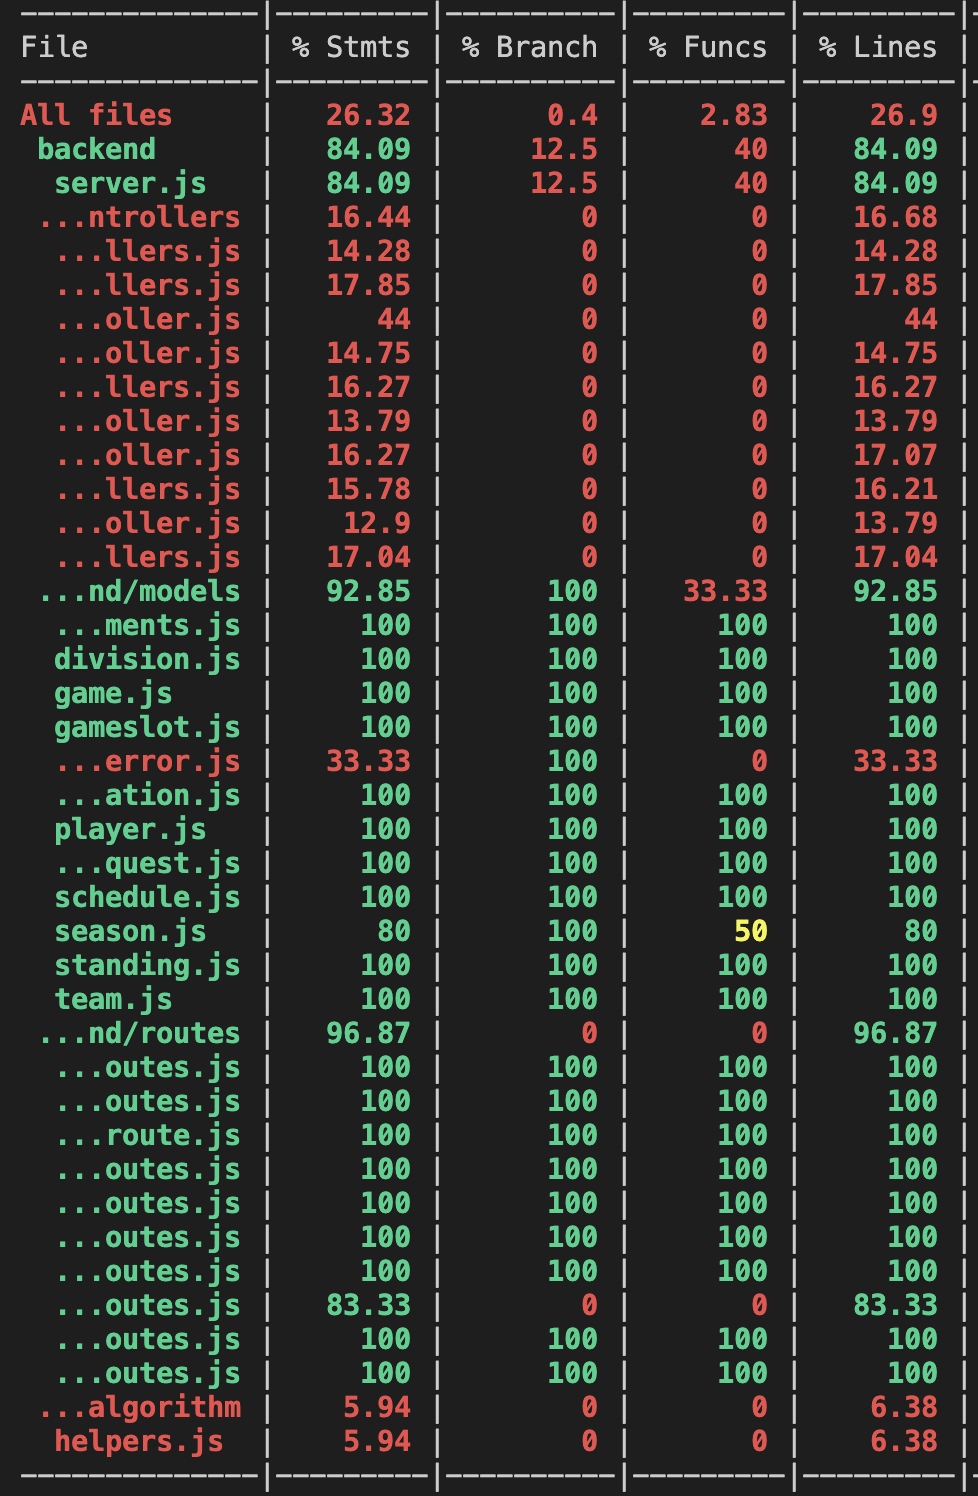
\includegraphics[width=\textwidth]{coverage.png}
    \label{fig:coverage}
\end{figure}

\bibliographystyle{plainnat}
\bibliography{../../refs/References}

\newpage{}
\section*{Appendix --- Reflection}

The information in this section will be used to evaluate the team members on the
graduate attribute of Reflection.

The purpose of reflection questions is to give you a chance to assess your own
learning and that of your group as a whole, and to find ways to improve in the
future. Reflection is an important part of the learning process.  Reflection is
also an essential component of a successful software development process.  

Reflections are most interesting and useful when they're honest, even if the
stories they tell are imperfect. You will be marked based on your depth of
thought and analysis, and not based on the content of the reflections
themselves. Thus, for full marks we encourage you to answer openly and honestly
and to avoid simply writing ``what you think the evaluator wants to hear.''

Please answer the following questions.  Some questions can be answered on the
team level, but where appropriate, each team member should write their own
response:


\begin{enumerate}
  \item What went well while writing this deliverable?
  
  The process of gathering and documenting test cases went smoothly, particularly due to the VnV Plan that we created previously to look back onto and the effective communication with the team. The detailed structure for each test case was already there, so we just had to follow our original plan and that really helped streamline the writing process.
  
  \item What pain points did you experience during this deliverable, and how
    did you resolve them?
    
    One challenge we had was adapting to the requirements from our supervisor, which led to the adjustments in the test cases throughout development. We resolved this by maintaining flexibility in our code approach and updating our test plans to adjust for those implementation changes. Overall, there weren't too many issues that were a pain to deal with.
     
  \item Which parts of this document stemmed from speaking to your client(s) or
  a proxy (e.g. your peers)? Which ones were not, and why?
  
  As mentioned before, the changes to test cases came directly from adapting to the requirements from our supervisor over the course of many meetings. One good example is FR-6 in our original VnV Plan, which was the player's ability to request to join a team. Our supervisor thought it would be annoying for captains to see many team invites, as players could just constantly request to join all the teams. Therefore, he asked us to remove the functionality completely to only allow captains to invite players they wanted. Some other parts of the documents were changed purely by our own thoughts and opinions, such as removing the need for captains to input game results (Win/Lose/Tie) in FR-8. We decided that it was a good change to improve the user experience, and speed up the process for captains to submit scores.
  
  \item In what ways was the Verification and Validation (VnV) Plan different
  from the activities that were actually conducted for VnV?  If there were
  differences, what changes required the modification in the plan?  Why did
  these changes occur?  Would you be able to anticipate these changes in future
  projects?  If there weren't any differences, how was your team able to clearly
  predict a feasible amount of effort and the right tasks needed to build the
  evidence that demonstrates the required quality?  (It is expected that most
  teams will have had to deviate from their original VnV Plan.)
  
  We have already discussed the modifications in the plan in the previous questions above, so we won't bother discussing it again in this section. Our VnV Plan originally had automated testing, but we had to deviate from that due to the superiority of manual testing for this website. It was extremely easy to test features, such as adding players to a team and verifying by looking at the database manually. 
  
  We've set the basis up of automated testing using Jest and connected CI to it, but it is not entirely complete at this deliverable checkpoint. Further, the unit testing plan was slightly different from the actual activities conducted for VnV. We've removed a few unit tests that were decided to be better tested manually or in system tests, and added some unit tests that we deemed necessary for the foundation of our application.

  The rest of our VnV Plan did not have to change, so there weren't many differences. Our team was able to clearly predict the right tasks to build the evidence that demonstrated the required quality because we have tremendous experience with sports platforms, participating in sports all our lives. Ever since coming to McMaster, we have regularly used McMaster IMLeagues to play intramurals, and we understand what makes a sports platform perform well from the users perspective. We also have experience with full-stack web development from our previous co-ops and internships, and we are familiar with building a big project from scratch. Testing was often regularly done before pushing our products to production.
  
\end{enumerate}

\end{document}